% Street-view country classification: a write-up of the Summer 2026 Deep Learning
% course project, written by Xiaochuan Li (28 Sep 2026). Every number is taken from the
% committed results of github.com/xchuan-li/HAI_DL_Group_Assignment (JSON histories,
% confusion matrix, results/README.md); figures are drawn by make_figs.py from data/.
% No new runs were made.
\documentclass[11pt,a4paper]{article}
\usepackage[T1]{fontenc}
\usepackage{newtxtext,newtxmath}
\usepackage[a4paper,margin=2.6cm]{geometry}
\usepackage{graphicx,booktabs,tikz,caption,microtype}
\usepackage[round]{natbib}
\usepackage[hidelinks]{hyperref}
\usetikzlibrary{positioning,arrows.meta}
\captionsetup{font=small,labelfont=bf}
\setlength{\parskip}{0.3em}
\definecolor{acc}{HTML}{17457A}

\title{\vspace{-1.2em}\textbf{Training Choices in a Small CNN for\\Street-View Country Classification}}
\author{Xiaochuan Li\\[0.2em]\small University of Technology Nuremberg \quad \texttt{xiaochuan.li@utn.de}}
\date{\small Written up September 2026 from a team course project, Deep Learning, Summer 2026\\
Code and results: \url{https://github.com/xchuan-li/HAI_DL_Group_Assignment}}

\begin{document}
\maketitle

\begin{abstract}
\noindent
We train a convolutional network from random initialisation to tell which of 18 countries a street image was taken in, with at most five million parameters and no external data. Instead of changing the architecture, we ask how far training choices alone move a fixed VGG-style network with 1.69 million parameters. Across 17 single-seed runs, validation accuracy rises from 0.619 to 0.823 (chance: 0.056). Four findings stand out. Fixing the training recipe (resolution, augmentation, schedule) gained 15.8 points on its own. An auxiliary coordinate target helped only while the model was under-trained. Regularisation interacted with training length: dropout 0.5 was the worst setting at 80 epochs and the best at 150. And a heuristic we steered by, that a best epoch at the very end of the schedule means the schedule is too short, failed when training for 250 epochs did worse than 200. Differences of a few images are treated as single-seed noise.
\end{abstract}

\section{Introduction}
Street images carry many cues to where they were taken: vegetation, road markings, architecture, signage, the colour of the soil. Telling countries apart from them is a hard fine-grained problem, and large geolocation systems rely on very large models and datasets \citep{planet}. This project had the opposite constraints: 10,800 labelled course images, no external data, a limit of five million parameters, and training from scratch.

Under these constraints we fixed a small backbone early and studied the training procedure instead: input resolution, augmentation, dropout, mixup, the optimiser, the length of the schedule, and how the output is formulated. After the first recipe change, every run changes one variable against a named reference, so each difference can be attributed. The aim was to learn which choices matter for a small network, and which apparent gains disappear under a fairer comparison.

\section{Data and evaluation}
The data are 10,800 labelled street images from 18 countries, 600 per country, each with the latitude and longitude at which it was taken. We split them 90/10, stratified by country with a fixed seed: 9,720 training and 1,080 validation images, exactly 60 per country, so per-country counts are directly comparable. A further 2,700 images form the course's hidden test set; their labels were never available to us, so every number here is validation accuracy on the fixed split. Chance is $1/18 = 0.056$, and one validation image is worth 0.0009.

\section{Model and training}
\begin{figure}[t]
\centering
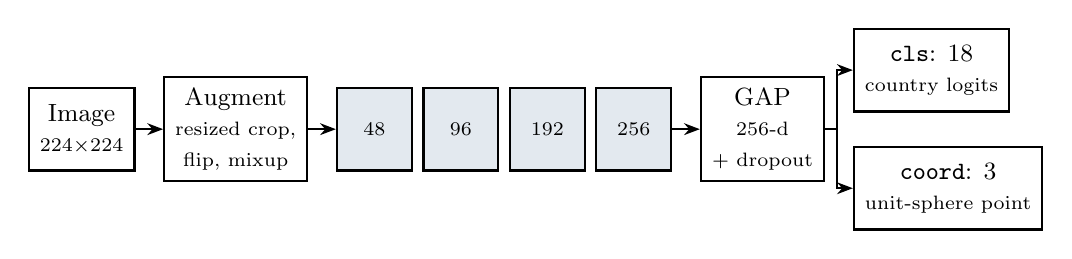
\begin{tikzpicture}[
  box/.style={draw, thick, minimum height=1.05cm, align=center, font=\small, inner sep=4pt},
  blk/.style={draw, thick, fill=acc!12, minimum height=1.05cm, minimum width=0.95cm, align=center, font=\scriptsize},
  arr/.style={-{Stealth[length=2mm]}, thick}, node distance=0.35cm]
\node[box] (img) {Image\\\scriptsize 224$\times$224};
\node[box, right=of img] (aug) {Augment\\\scriptsize resized crop,\\\scriptsize flip, mixup};
\node[blk, right=of aug] (b1) {48};
\node[blk, right=0.12cm of b1] (b2) {96};
\node[blk, right=0.12cm of b2] (b3) {192};
\node[blk, right=0.12cm of b3] (b4) {256};
\node[box, right=of b4] (gap) {GAP\\\scriptsize 256-d\\\scriptsize + dropout};
\node[box, right=of gap, yshift=0.75cm] (cls) {\texttt{cls}: 18\\\scriptsize country logits};
\node[box, right=of gap, yshift=-0.75cm] (reg) {\texttt{coord}: 3\\\scriptsize unit-sphere point};
\draw[arr] (img) -- (aug); \draw[arr] (aug) -- (b1); \draw[arr] (b4) -- (gap);
\draw[arr] (gap.east) -- ++(0.15,0) |- (cls.west); \draw[arr] (gap.east) -- ++(0.15,0) |- (reg.west);
\end{tikzpicture}
\caption{The network, 1,685,253 parameters (34\% of the limit). Each shaded block is two 3$\times$3 convolution--BatchNorm--ReLU layers and max-pooling; the numbers are channel widths. Both heads read the same pooled feature vector. Which head is trained, and which one decides, depends on the mode: \texttt{cls} (classification only), \texttt{multi} (classification plus a coordinate loss) or \texttt{regress} (coordinates only, nearest country centroid). The submitted model uses \texttt{cls}.}
\label{fig:model}
\end{figure}

\paragraph{Architecture.} The backbone (Figure~\ref{fig:model}) follows the VGG pattern \citep{vgg}: four blocks of two 3$\times$3 convolution--batch normalisation--ReLU layers \citep{bn} and max-pooling, with widths 48, 96, 192 and 256. Global average pooling \citep{nin} replaces a flattened fully connected layer, which keeps the model small and makes its size independent of input resolution, so the 112- and 224-pixel runs compare the same network. Dropout \citep{dropout} acts on the pooled 256-dimensional vector, after every batch-normalisation layer, so that it does not disturb the normalisation statistics. Two linear heads read this vector: 18 country logits, and a three-dimensional point normalised onto the unit sphere and regressed against the photo's true location. The coordinate head exists in every mode, so the backbone and parameter count are identical across modes.

\paragraph{Training.} The submitted model is trained in the \texttt{cls} mode at 224$\times$224 pixels (the originals are 512 pixels), with random resized crops and horizontal flips, dropout 0.5, mixup with $\alpha = 0.2$ \citep{mixup}, Adam \citep{adam} with learning rate $10^{-3}$, weight decay $10^{-4}$ and batch size 256, an eight-epoch warm-up \citep{goyal} followed by cosine decay \citep{sgdr}, for 200 epochs. Colour jitter is deliberately off, since colour (red soil, vegetation, haze) is itself a geographic cue. There is no test-time augmentation or ensembling, so the reported accuracy is that of the submitted model. The labelled images are decoded once, held in GPU memory as 8-bit arrays, and augmented there in batches; an epoch takes about 14 seconds, and the final run 47.9 minutes on one NVIDIA A40. This pipeline was written by a teammate (see Contributions).

\section{Experiments}
We made 17 runs, all with the same seed. Figure~\ref{fig:progress} summarises the path to the submitted model; the subsections take each step in turn.

\begin{figure}[h]
\centering
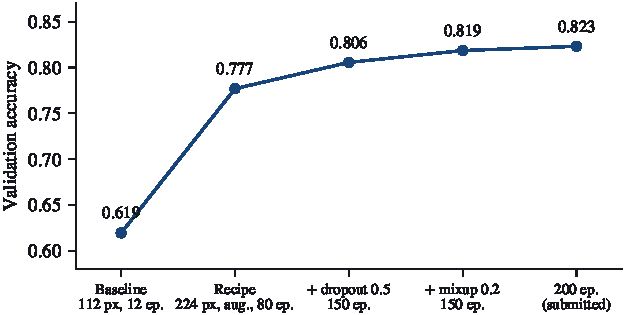
\includegraphics[width=0.8\linewidth]{figs/progression.pdf}
\caption{Best validation accuracy after each step. Chance is 0.056, below the plotted range.}
\label{fig:progress}
\end{figure}

\subsection{The training recipe mattered more than anything else}
The first baseline was deliberately minimal: 112-pixel inputs, no augmentation, twelve epochs at a flat learning rate. Changing only the recipe (224 pixels, random resized crops and flips, 80 epochs with a five-epoch warm-up and cosine decay) raised accuracy from 0.619 to 0.777 with the architecture untouched. The gains landed where the baseline's confusion matrix predicted: countries near chance improved most (Argentina 7 to 37 of 60, India 21 to 51, the United States 16 to 41), countries already near ceiling barely moved (Iceland 55 to 55, Canada 45 to 47), and a baseline cluster of confusions among arid countries dissolved (India predicted as Egypt: 15 to 0). We did not separate resolution, augmentation and schedule, so we cannot say how the gain divides among them.

\begin{figure}[h]
\centering
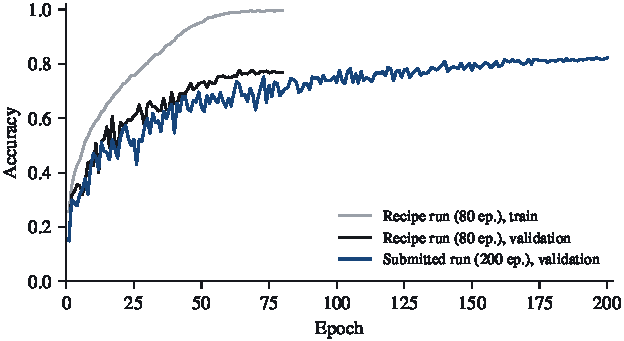
\includegraphics[width=0.8\linewidth]{figs/curves.pdf}
\caption{Learning curves. In the 80-epoch recipe run, training accuracy passes 0.99 at epoch 65 while validation stays near 0.77: the remaining epochs mostly memorise. The submitted run's training accuracy is not shown, since under mixup it is scored against blended inputs and is not comparable.}
\label{fig:curves}
\end{figure}

\paragraph{Overfitting became the binding constraint.} At 0.777 the model reached 0.996 training accuracy against 0.777 on validation (Figure~\ref{fig:curves}), a gap of 22 points with augmentation already on. Capacity and resolution were no longer the bottleneck; regularisation was.

\subsection{Regularisation, and how it interacts with training length}
\begin{figure}[h]
\centering
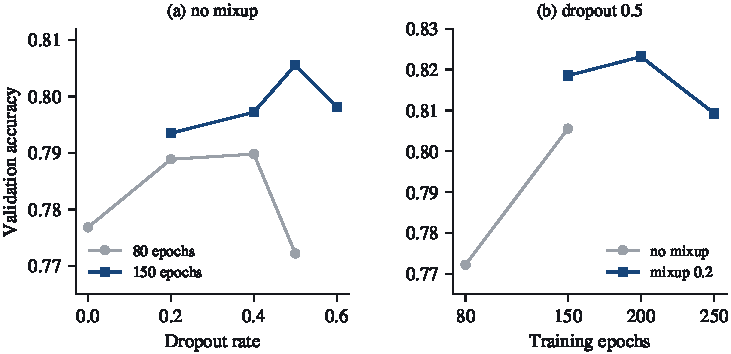
\includegraphics[width=0.9\linewidth]{figs/sweeps.pdf}
\caption{(a) Dropout rate at two schedule lengths, without mixup. (b) Schedule length at dropout 0.5, with and without mixup. Each axis has an interior optimum, and where it lies depends on the other setting.}
\label{fig:sweeps}
\end{figure}

\paragraph{Dropout.} At 80 epochs, dropout 0.2 and 0.4 performed within one image of each other (0.789 and 0.790), and dropout 0.5 fell to 0.772, below no dropout at all (Figure~\ref{fig:sweeps}a). At 150 epochs, 0.5 was the best setting (0.806). The same rate was thus the worst setting at one schedule length and the best at another: a longer schedule gives the model more room to memorise, so it both tolerates and needs more regularisation. The failure at 0.5 over 80 epochs also shows how over-regularisation fails. Its train--validation gap (0.176) matched that of 0.4, but training accuracy fell from 0.966 to 0.949 and validation fell with it: past a point, regularisation stops trading training fit for generalisation and simply removes capacity.

\paragraph{Mixup.} Mixup with $\alpha = 0.2$ added 14 images on top of dropout 0.5 (0.819) and 21 on top of dropout 0.4 (0.817). We had expected it to over-regularise, since 0.5 was already the peak of the dropout curve. Instead, the difference between the two dropout rates shrank from 9 images without mixup to 2 with it: mixup replaced part of what dropout supplied rather than adding to it. Regularisers that act in different places, the data distribution and the features, do not simply sum.

\paragraph{Optimiser.} Replacing Adam with AdamW \citep{adamw}, everything else fixed, gave 0.800 against 0.806, six images fewer. Best epoch (122 vs.\ 125) and final training accuracy (0.993 vs.\ 0.995) agree as well; at a weight decay of $10^{-4}$ the two optimisers behave alike. Testing this first, as the simplest single variable, would have forced a decision on a six-image difference.

\paragraph{Training length, and a heuristic that failed.} At the final settings, 150 epochs gave 0.819, 200 gave 0.823 and 250 gave 0.809, fifteen images fewer than 200 (Figure~\ref{fig:sweeps}b). Until then we had read a best epoch at the very end of the schedule as a sign that the schedule was too short, and extended it four times on that basis. But the best epochs of these three runs were 143/150, 196/200 and 241/250: at the end every time, including the run that is clearly too long. Under cosine decay the learning rate approaches zero at the end, so validation accuracy peaks there almost regardless of length. The heuristic is informative in one direction only: the unregularised 80-epoch run peaked at epoch 64 and then stayed flat, which is a real sign of saturation.

\subsection{How the output is formulated}
\begin{figure}[h]
\centering
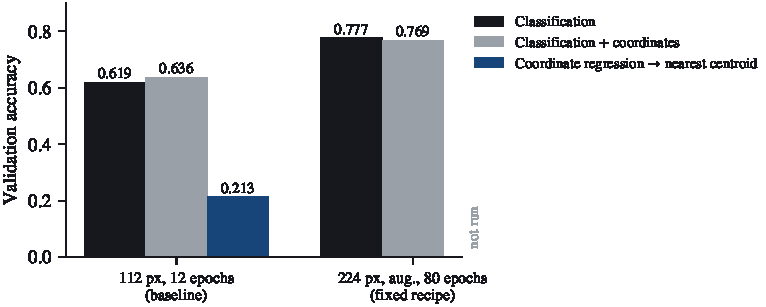
\includegraphics[width=0.85\linewidth]{figs/heads.pdf}
\caption{Three output formulations. The advantage of the auxiliary coordinate target at the baseline disappears once the recipe is fixed. Regression was only run at the baseline.}
\label{fig:heads}
\end{figure}

With backbone, initialisation, data order and schedule held fixed, we compared the three modes (Figure~\ref{fig:heads}). At the 112-pixel baseline, classification reached 0.619, classification with the auxiliary coordinate loss 0.636, and pure coordinate regression 0.213.

\paragraph{The auxiliary target helped only an under-trained model.} After the recipe was fixed, the auxiliary target no longer helped: 0.769 against 0.777 for classification alone, a nine-image difference within single-seed noise. The extra supervision had helped a model that had not yet learned enough from its labels. Had we stopped at the baseline, we would have kept the auxiliary head for the wrong reason; an ablation is only informative on top of a properly trained baseline.

\paragraph{Coordinate regression fails for a structural reason.} Under a squared loss, a regressor predicts the average of the plausible locations. When an image is ambiguous, that average lies between candidates, often at sea or inside a neighbour, and the nearest-centroid rule then collapses whole regions onto the most central country: New Zealand was assigned to Papua New Guinea in 30 of 60 cases, Egypt to Saudi Arabia in 28, Canada to Mexico in 24. Borders are also invisible in coordinates. Measured against the spherical centroids the rule uses, the mean distance from an image to its own country's centroid is 1,401\,km for the United States and 1,529\,km for Canada, while the two centroids lie 1,502\,km apart: the spread within a country is as large as the separation between countries. Classification keeps its decision on a real country and can use appearance cues that coordinates cannot express, which is also why large geolocation systems treat the task as classification \citep{planet}.

\subsection{Where the submitted model still fails}
\begin{figure}[h]
\centering
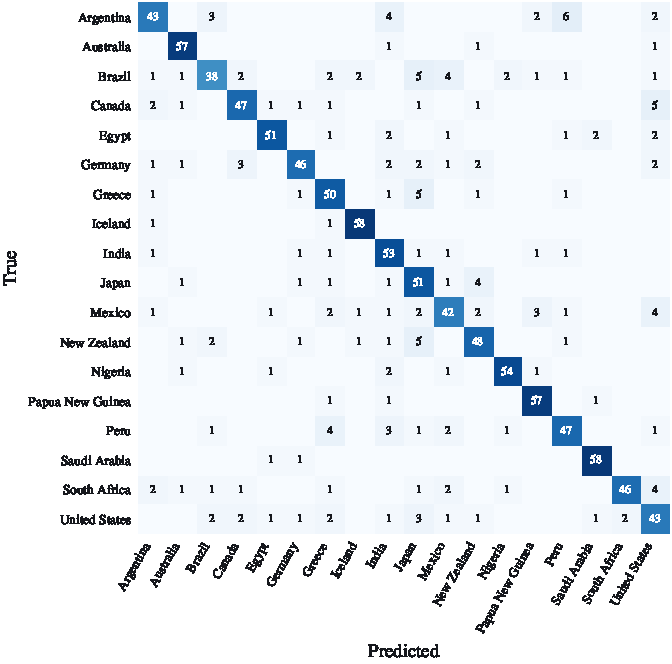
\includegraphics[width=0.58\linewidth]{figs/confusion.pdf}
\caption{Confusion matrix of the submitted model on the 1,080 validation images (60 per country; darker is more).}
\label{fig:confusion}
\end{figure}

The submitted model classifies 889 of 1,080 validation images correctly (Figure~\ref{fig:confusion}). The weakest countries are Brazil (38 of 60), Mexico (42), Argentina and the United States (43 each); the strongest are Iceland and Saudi Arabia (58 each), Australia and Papua New Guinea (57 each). The largest remaining confusions are small and scattered: Argentina as Peru (6), and New Zealand, Greece and Brazil as Japan, and Canada as the United States (5 each). Several of these pair countries with similar landscapes or road environments, but we did not analyse the images behind them.

\section{Discussion}
Within a fixed small architecture, the training procedure moved validation accuracy by 20 points, from 0.619 to 0.823. Most of what we learned concerns comparisons rather than settings: an optimal hyperparameter under one schedule was not optimal under another; an auxiliary target's advantage came from comparing against an under-trained baseline; two regularisers partly substituted for each other; and a reasonable-looking stopping heuristic failed exactly once, in the case that mattered.

\paragraph{Limitations.} Every run uses a single seed, so differences of about ten images or fewer should not be read as reliable. All numbers are validation accuracies on one split, and the submitted configuration was selected on that same split, so its accuracy is an optimistic estimate of test performance; the hidden test labels were never available. The recipe step changed three factors at once. We made no new runs for this write-up.

\section*{Contributions}
This was a three-person course project. A teammate designed and implemented the training pipeline, including the in-memory data handling; another compiled the results for the course report. I trained the models, ran the experiments described here, and analysed validation performance and confusion matrices. The analyses in this write-up come from the project's committed results and experiment record; the text and figures are my own and were prepared after the course.

\begin{thebibliography}{10}\small
\bibitem[Goyal et al.(2017)]{goyal} P.~Goyal, P.~Doll\'ar, R.~Girshick, et al. Accurate, large minibatch SGD: Training ImageNet in 1 hour. \emph{arXiv:1706.02677}, 2017.
\bibitem[Ioffe and Szegedy(2015)]{bn} S.~Ioffe and C.~Szegedy. Batch normalization: Accelerating deep network training by reducing internal covariate shift. In \emph{ICML}, 2015.
\bibitem[Kingma and Ba(2015)]{adam} D.~P.~Kingma and J.~Ba. Adam: A method for stochastic optimization. In \emph{ICLR}, 2015.
\bibitem[Lin et al.(2014)]{nin} M.~Lin, Q.~Chen, and S.~Yan. Network in network. In \emph{ICLR}, 2014.
\bibitem[Loshchilov and Hutter(2017)]{sgdr} I.~Loshchilov and F.~Hutter. SGDR: Stochastic gradient descent with warm restarts. In \emph{ICLR}, 2017.
\bibitem[Loshchilov and Hutter(2019)]{adamw} I.~Loshchilov and F.~Hutter. Decoupled weight decay regularization. In \emph{ICLR}, 2019.
\bibitem[Simonyan and Zisserman(2015)]{vgg} K.~Simonyan and A.~Zisserman. Very deep convolutional networks for large-scale image recognition. In \emph{ICLR}, 2015.
\bibitem[Srivastava et al.(2014)]{dropout} N.~Srivastava, G.~Hinton, A.~Krizhevsky, I.~Sutskever, and R.~Salakhutdinov. Dropout: A simple way to prevent neural networks from overfitting. \emph{JMLR}, 15:1929--1958, 2014.
\bibitem[Weyand et al.(2016)]{planet} T.~Weyand, I.~Kostrikov, and J.~Philbin. PlaNet: Photo geolocation with convolutional neural networks. In \emph{ECCV}, 2016.
\bibitem[Zhang et al.(2018)]{mixup} H.~Zhang, M.~Cisse, Y.~N.~Dauphin, and D.~Lopez-Paz. mixup: Beyond empirical risk minimization. In \emph{ICLR}, 2018.
\end{thebibliography}
\end{document}
